\subsection{Hit Reconstruction Efficiency}
\label{sec:Systematics_HitEfficiency}

We use a side-band sample of beam events to evaluate 
the layer by layer hit reconstruction efficiency in the \p0d. The sample is generated by looking at events originating in the first layer of the P0D and is not a part of the actual selection. 
The hit reconstruction efficiency combines both the probability of finding an above threshold hit 
in a \p0d bar with the probability of reconstructing succesfully combining 
the hit into a track. 
As the \p0d Reconstruction algorithm allows for gaps of hits in a track, 
we use particularly long reconstructed tracks to evaluate 
the rate of missed layers. 
Since each \p0dule has two layers (an X and a Y layer), 
we expect any track passing through a \p0dule to create 
two reconstructed nodes. 
So for each reconstructed track, we use the most upstream node 
and the most downstream node to calculate the number of total expected nodes. 
This value is compared to the number of actually reconstructed nodes. 
Then the efficiency per layer is given 
by: $($\# Expected Nodes - \# Reconstructed Nodes$)/($\# Expected Nodes$)$. 
To have similar levels of \p0d bar coverage in both Data and MC, 
we also require that any tracks used in this study begin and end at similar layer ranges. 
The hit reconstruction efficiency as a function of layer number 
is shown in Figure \ref{fig:hiteffsand}.

\begin{figure}
\centering
\includegraphics[width=2.5in]{Figures/Systematics/HitEfficiency/Hiteffsandw.eps}
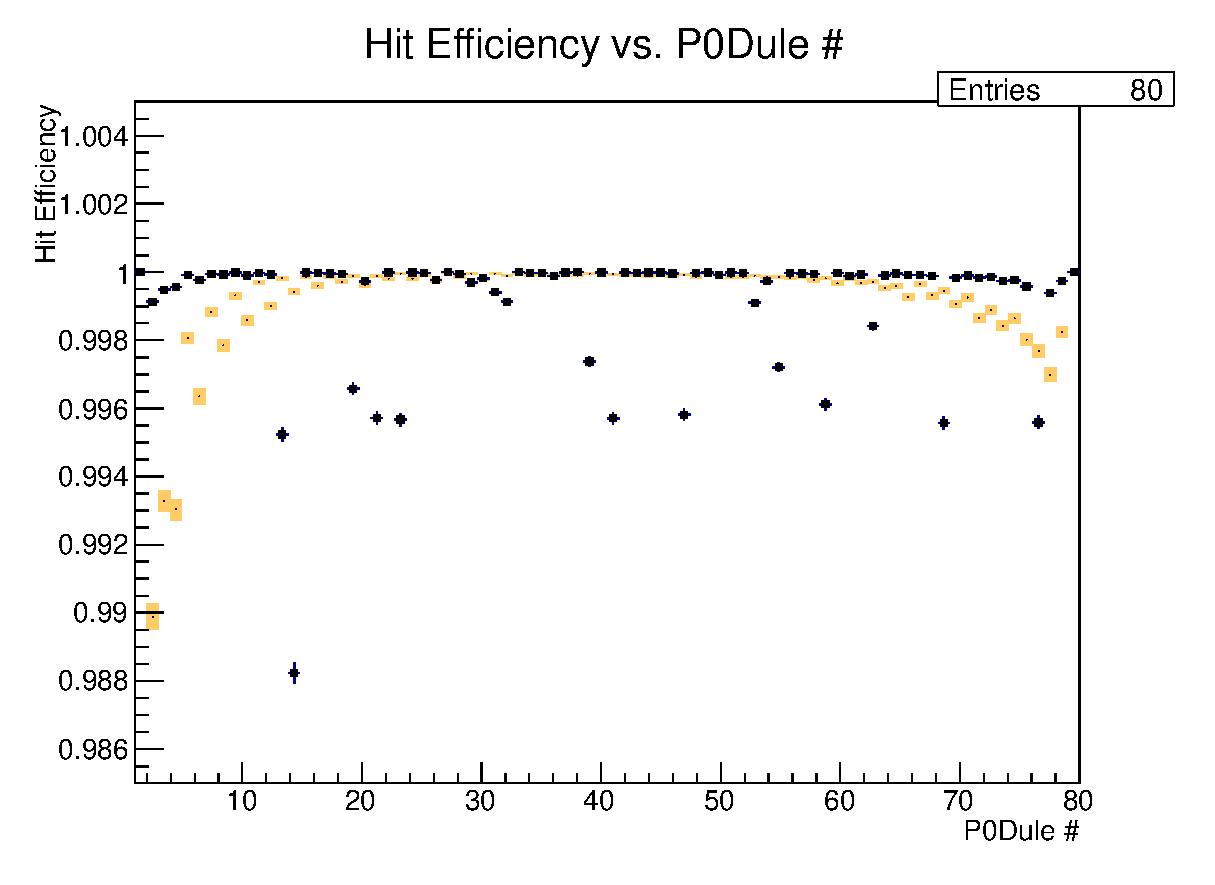
\includegraphics[width=2.5in]{Figures/Systematics/HitEfficiency/Hiteffsanda.eps}
\caption{The hit reconstruction efficiency as a function of layer number for water-in running (left) and water-out running (right). Data (black dots with error bars) and MC (orange error bars) show very high efficiencies for all layers. Layers corresponding to the water target have almost perfect efficiency. A few layers in the water target have ~0.5\% inefficiency. Note that the Y-axis is zero-suppressed.}
\label{fig:hiteffsand}
\end{figure}

\begin{table}
\centering
\begin{tabular}{lcccc}\toprule\midrule
Layer \# &  Data (Water). & MC (Water) & Data (Air) & MC (Air)  \\ \midrule
15 & 1 & 0.999894 & 0.999984 & 0.999857 \\ \midrule
65 & 0.999916 & 0.999718 & 0.99996 & 0.999587 \\ \midrule
77 & 0.999638 & 0.998028 & 0.995591 & 0.997677 \\ \midrule
78 & 0.999359 & 0.998028 & 0.999394 & 0.996979 \\ \midrule
79 & 0.999638 & 0.998416 & 0.99975 & 0.998247 \\ \midrule
%80 & 0.994044 & 0.999141  \\ \midrule
\bottomrule
\end{tabular}
\caption{Data and MC hit reconstruction efficiencies by relevant layer numbers. Errors are excluded as the efficiencies are so high. }
\label{tab:hiteff}
\end{table}


As expected, the hit reconstruction is extremely high. The few layers in Data with small ~0.5\% inefficiencies are at the single bar level, which are also expected. Any systematic arising from hit reconstruction efficiency will feed in through our matching algorithm and the Fiducial Volume cut. In the matching algorithm, we require that the \p0d track have a node in the last two p0dules, so if both p0dules somehow failed to reconstruct a node, then we would have a small inefficiency. This last two p0dules correspond to layer numbers 77-80. Also, when making the fiducial volume cut, we may misreconstruct out-of-FV tracks as in-FV due to missed nodes at the upstream end of the water target. Similarly, we may lose in-FV tracks in the downstream end of the water target. Even in the least efficient of our p0dules, failing to reconstruct two or more adjacent nodes from a track is negligible (less than 0.0025\%), so we can estimate the effect of hit reconstruction efficiency on the fiducial cut using only the likelihood of missing a single node. The upstream end of the fiducial volume corresponds to layer 15 and the downstream end corresponds to layer 65. The hit reconstruction efficiencies for layers 15, 65, and 77-80 are given in Table \ref{tab:hiteff}.

From this table, we can then extract the final systematic values due to hit reconstruction efficiency. The probability of having NO nodes in the last two layers is essentially zero and therefore not included as a systematic. The probability of having gained an out-of-FV track from the upstream end of the FV cut is given by number of muon candidate tracks originating in layer 16 multiplied by the inefficiency of layer 15. Similarly, the probability of having missed an in-FV track at the downstream end of the FV cut is given by the \# of muon candidate tracks orginating in layer 66 multiplied by the inefficiency of layer 65. The largest inefficiency is that from layer 65 in MC air running, and it is 0.04$\%$. As the change in the Data/MC ratio due to gains and losses of events from hit inefficiency cannot exceed this fraction, and is realistically smaller, we can neglect any systematic effect from hit efficiency differences between Data and MC.

\subsubsection{Neutral Back Scattering}

To be able to apply the layer efficiency study 
(Sec. \ref{sec:Systematics_HitEfficiency})
on our \p0d+TPC1 CC inclusive samples, we have preformed a similar 
layer by layer efficiency study with the CC inclusive samples. 
The efficiency study have yielded, as expected, 
very high layer efficiencies for 
both Data and MC samples.
In addition the study found that for 
a certain number of times in both beam Data and MC, 
we observe 
%large 
near the start of a track a node gaps, which is larger than 1 node.
% near the start of a track. 
We investigated these set of tracks and identified these 
gaps not to be related to layers inefficiencies. 
The investigations have found that these tracks are 
cases were an event had a
%that are not related to hit reconstruction inefficiencies. 
%Using MC, these events have been confirmed as 
neutral particle, which was back scattered from 
the interaction and converted several layers upstream 
of the true interaction vertex. 
As a result the additional hits from the converted neutral particle 
have been added to a forward going track. 
%reconstructed together with the track, 
%These additional hits have
This effect have caused the track start position to migrate  
to a an upstream location and to add layers gap in between.\\

We have further studied and looked at different properties of this topology. 
Tables \ref{tab:NodeMissFractionsWaterIn} 
and \ref{tab:NodeMissFractionsWaterOut} shows for different samples 
the fraction of tracks that have more than 1 node missed normalized 
to the number of tracks in that sample.
%Our study 
%These investigations have showed 
%have shown that 
%rates of tracks with more than 1 missing node are consistent between 
%our Data and MC samples. The 
%The fractions of tracks with more than 1 node missed 
%in Run 1 Data and MC samples are $0.90\%$ and $1.38\%$ 
%for Data and MC 
%respectively. 
For Run 1 we have found that the Data and MC fractions 
are $0.90\%$ and $1.38\%$ respectively. 
Similar behavior between Data and MC is seen at the Run 2 period 
were the fractions are $1.08\%$ and $1.40\%$ for Data and MC respectively. 
We use these fractions to find the amount in which the MC 
should be corrected, to mimic the Data, for both run periods.
The correction values we extracted are 0.13 and 0.16 events for 
Run 1 and Run 2 respectively. \\

\begin{table}[h]
\centering
\begin{tabular}{lcc}\toprule
      & &  Fraction of tracks \\
\cline{2-3}
Run 1 & Data & $1.63\%$  \\ 
      & MC & $1.90\%$  \\ 
\cline{2-3}
Run 2 & Data & $1.40\%$  \\ 
      & MC & $1.76\%$ \\ 
\cline{2-3}
Run 4 & Data & $1.39\%$  \\ 
      & MC & $1.80\%$ \\ 
\bottomrule
\end{tabular}
\caption{The fractions of tracks with more than 1 missed node 
for both Data and MC Water-in samples in the different run periods.}
\label{tab:NodeMissFractions}
\end{table}

\begin{table}[h]
\centering
\begin{tabular}{lcc}\toprule
      & &  Fraction of tracks \\
\cline{2-3}
Run 2 & Data & $1.55\%$  \\ 
      & MC & $1.83\%$  \\ 
\cline{2-3}
Run 3 & Data & $1.46\%$  \\ 
      & MC & $1.80\%$ \\ 
\cline{2-3}
Run 4 & Data & $1.65\%$  \\ 
      & MC & $1.80\%$ \\ 
\bottomrule
\end{tabular}
\caption{The fractions of tracks with more than 1 missed node 
for both Data and MC Water-out samples in the different run periods.}
\label{tab:NodeMissFractionsWaterOut}
\end{table}

\begin{figure}
\centering
\includegraphics[width=2.5in]{Figures/layerEff-5F5E-Run1-ccinc-DoMC-MissedLayerPerTracks.eps}
\includegraphics[width=2.5in]{Figures/layerEff-5F5E-Run2air-ccinc-DoMC-MissedLayerPerTracks.eps}
\includegraphics[width=2.5in]{Figures/layerEff-5F5E-Run2-ccinc-DoMC-MissedLayerPerTracks.eps}
\includegraphics[width=2.5in]{Figures/layerEff-5F5E-Run3air-ccinc-DoMC-MissedLayerPerTracks.eps}
\includegraphics[width=2.5in]{Figures/layerEff-5F5E-Run4-ccinc-DoMC-MissedLayerPerTracks.eps}
\includegraphics[width=2.5in]{Figures/layerEff-5F5E-Run4air-ccinc-DoMC-MissedLayerPerTracks.eps}
\caption{Layers distance from the first layer of missed nodes normalized 
to the number of tracks. 
The left columnb shows Water-in periods, from top to bottom 
are Run 1, Run 2 and Run 4.  
The right columb shows Water-out periods, from top to bottom 
are Run 2, Run 3 and Run 4.
In all periods 
the blue and red histograms are generated from the Data and MC samples
respectively.
}
\label{fig:MisssedNodePerTracks}
\end{figure}

Another studied aspect 
%that was studied 
was 
%the length at which the convertion occurs.
the distance of missed layers with respect to 
the first layer, the start of the track.
Fig. \ref{fig:MisssedNodePerTracks} shows the results of this study. 
%which is the frequent of a missed layer as a function of distance 
f%rom the first layer. 
The figure presents the 
missed layers distributions for both  
Data and MC samples, normalized to the number of available tracks.
One can clearly identify that the second node, 
of the tracks that had missed layers, 
% samples studied 
has the highest missed frequently. 
Another feature is the 'missed node' peak around layer 10 with 
the spread between 5 to 20 layers. 
It seem that the MC samples mimics the Data distribution 
of this feature.
Followed this spread we have calculated the number of tracks 
with missed layers, 5 to 20 layers from the start of the track 
for both run periods. 
These rates per POT are summarized 
in Tables \ref{tab:TracksWithMiss0to20perPTWaterIn} 
and \ref{tab:TracksWithMiss0to20perPTWaterOut}.
From this table one can see that the rates are similar 
between Data and MC. \\

\begin{table}[h]
\centering
\begin{tabular}{lcc}\toprule
      & &  Tracks per POT [$\times 10^{-18}$] \\
\cline{2-3}
Run 1 & Data & $6.53$  \\ 
      & MC & $7.92$ \\ 
\cline{2-3}
Run 2 & Data & $7.13$  \\ 
      & MC & $8.08$ \\ 
\cline{2-3}
Run 4 & Data & $7.52$  \\ 
      & MC & $8.12$ \\ 
\cline{2-3}
Run 1+2+4 & Data & $7.32$  \\ 
      & MC & $8.09$ \\ 
\bottomrule
\end{tabular}
\caption{The rate of tracks
with missed layers (layers 0 to 20 from counting from the start of the track)
for the Data and MC Water-in samples 
as calculated for Run 1, Run 2, Run 4 and Run 1$+$2$+$4 combined periods.
}
\label{tab:TracksWithMiss0to20perPTWaterIn}
\end{table}

\begin{table}[h]
\centering
\begin{tabular}{lcc}\toprule
      & &  Tracks per POT [$\times 10^{-18}$] \\
\cline{2-3}
Run 2 & Data & $5.38$  \\ 
      & MC & $6.34$ \\ 
\cline{2-3}
Run 3 & Data & $6.14$  \\ 
      & MC & $6.34$ \\ 
\cline{2-3}
Run 4 & Data & $5.80$  \\ 
      & MC & $6.34$ \\ 
\cline{2-3}
Run 2+3+4 & Data & $5.90$  \\ 
      & MC & $6.34$ \\ 
\bottomrule
\end{tabular}
\caption{The rate of tracks
with missed layers (layers 0 to 20 from counting from the start of the track)
for the Data and MC Water-out samples 
as calculated for Run 2, Run 3, Run 4 and Run 2$+$3$+$4 combined periods.
}
\label{tab:TracksWithMiss0to20perPTWaterOut}
\end{table}

All the above show that the skipped nodes/layers due to neutral particles 
is a small fraction of our CC inclusive sample. 
Moreover the frequencies and rates per POT of these effects 
in the MC samples look alike the Data distributions. 
These leads us to a very small systematic error contribution 
which was not included in the final summary table.

%Using beam Data and MC, we quantify both the rate of occurrence 
%of these backscattered events, as well as the characteristic length 
%at which these neutrals convert. 
%We then propagate this into an appropriate systematic 
%following the same prescription as hit reconstruction efficiency. 

